\section{Software Development}

\label{sec:coding}

\subsection{Software Design}

The engine for particle tracking on the GPU is built upon the solid particle library. A solver called \verb+gpuLagrangianFoam+ was developed. If it is invoked using the \verb+-gpu+ switch, tracking will be executed on the GPU. Because CUDA files must be compiled using Nvidia's proprietary compiler, \verb+nvcc+, the code using CUDA keywords was developed as a separate shared library against which the solver must be linked. The rest of the solver code can be compiled in the same way as any other OpenFOAM application.

\paragraph{Mesh Data}

As explained earlier, the OpenFOAM \verb+Cloud+ class stores particles in a linked list, which is not suitable for parallel processing on a GPU. Before the mesh can be used on the GPU, it is converted into a more suitable format, which is described here. Three dimensional vectors are padded to 4 elements such that they can be fetched using CUDA's built in vector data types \verb+float4+ or \verb+double4+. For example, the cell centres are stored by the order of cell labels as illustrated in figure \ref{gfx:cellCentres}.

\begin{figure}[H]
  \centering
  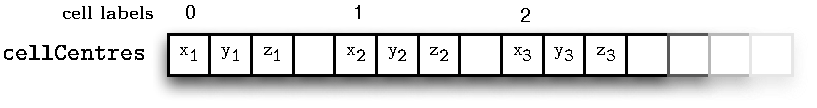
\includegraphics[scale=0.8]{content/gfx/cellCentres.pdf}
  \caption{Cell centres arranged in memory.}
  \label{gfx:cellCentres}
\end{figure}

The cell labels are not stored, since they go from $0$ to the number of cells $- 1$. Storing the face labels associated with the cell labels requires some more effort because in an unstructured mesh a cell can have any number of faces. 

\begin{figure}[H]
  \centering
  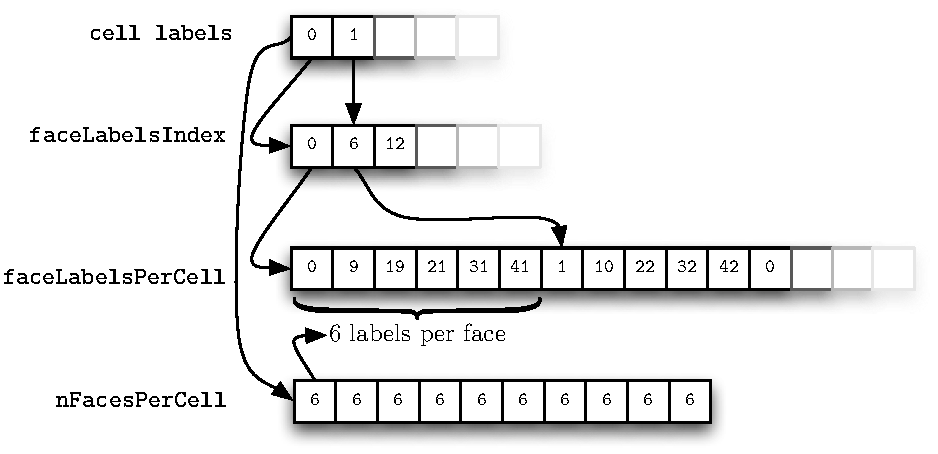
\includegraphics[scale=0.8]{content/gfx/cellFacesMapping.pdf}
  \caption{Mesh data layout in memory.}
  \label{gfx:cellFacesMapping}
\end{figure}

Figure \ref{gfx:cellFacesMapping} illustrates the mapping from the cell labels to the concerning face labels. The face labels are stored in the array \verb+faceLabelsPerCell+, by cell. Meaning that the first six face labels belong to cell \verb+0+ and the next six to cell \verb+1+. Face label \verb+0+ appears twice, this is the label of the face between cell \verb+0+ and \verb+1+. The \verb+faceLabelsIndex+ array stores the indices of the \verb+faceLabelsPerCell+ array, where the face labels to a given cell start. Note that the array names are identically to the ones used in the code. The mesh data was taken from the tunnel test case (see section \ref{sec:particleTunnel}), which consists of ten cubes placed one after another. Data belonging to a certain face, such as the face centres and the face normals are stored at the same index as the face labels. The neighbour and owner arrays are implemented as described in section \ref{sec:meshRepresentation}. This is illustrated in figure \ref{gfx:ownerNeighbour}, the data is again taken from the particle tunnel case. There are only ten faces with a neighbour cell: Face 0 has neighbour cell 1, face 1 neighbour cell 2 and so forth. 

\begin{figure}[H]
  \centering
  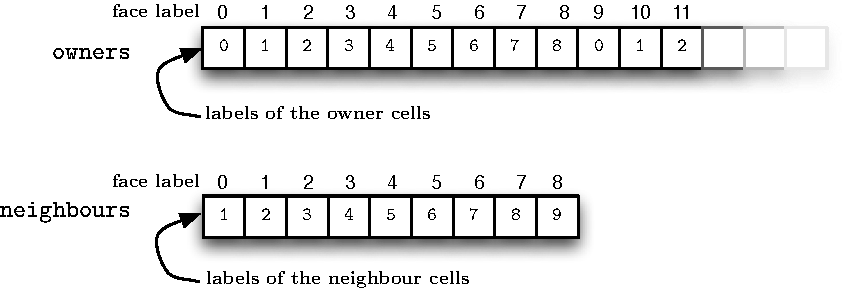
\includegraphics[scale=0.8]{content/gfx/ownerNeighbour.pdf}
  \caption{Owner and neighbour data of the particle tunnel case.}
  \label{gfx:ownerNeighbour}
\end{figure}

\paragraph{Particle Data}

The particle data is stored in a similar fashion as the mesh data. For example the labels of the faces for which $\lambda_c$ is in the interval $[0,1]$ (see section \ref{sec:particleTrackingAlgo}) also use an additional index array.

\paragraph{Abstraction and Data Encapsulation}

When programming CUDA, the host code can be completely written in C++ while only C code with a few extensions borrowed from C++ such as operator overloading or function templates \cite[Appendix D]{cudaguide} is allowed on the device. This makes it impossible to use containers from the C++ standard template library (STL) or OpenFOAM classes on the device. Using only manually allocated arrays in order to manage the data often leads to error prone code and therefore long testing and debugging time. To transform the data into a flat structure, suitable for the GPU, the vector container from the STL was used. The C++ ISO standard guarantees that the data is stored contiguously in memory such that it can be copied to the GPU using raw pointers. From the C++ standard document \cite[23.3.6.1]{cpp}:

\begin{quote}
The elements of a vector are stored contiguously, meaning that if \verb+v+ is a \verb+vector<T, Allocator>+ where \verb+T+ is some type other than bool, then it obeys the identity \verb@&v[n] == &v[0] + n@ for all \verb@0 <= n < v.size()@.
\end{quote}

The classes of the GPU particle engine use a wrapper which holds a reference to the concerning instance of \verb+std::vector+ and a pointer to the device memory as member variables. The wrapper class is called \verb+cuvector+. Device memory is allocated upon construction and freed when the destructor is called. Memory can be copied from the host to the device calling \verb+upload()+ on the cuvector object, \verb+download()+ is used to copy the data back from the device to the host memory. The code of the particle tracking engine is divided into three major classes: The \verb+FlatMesh+ class holds all the mesh data and does basic operations on it, such as figuring out what the cell next to another cell is, given a cell and a face label. The \verb+ParticleData+ class holds all particle related data. Finally the \verb+particleEngine+ class is derived from the \verb+ParticleData+ class and does the actual computation, such as computing all the $\lambda_c$ and the $\lambda_a$. It also moves particles and keeps track of how many particle do still need tracking. Figure \ref{gfx:engineOverview} illustrates these classes briefly.

\begin{figure}[H]
  \centering
  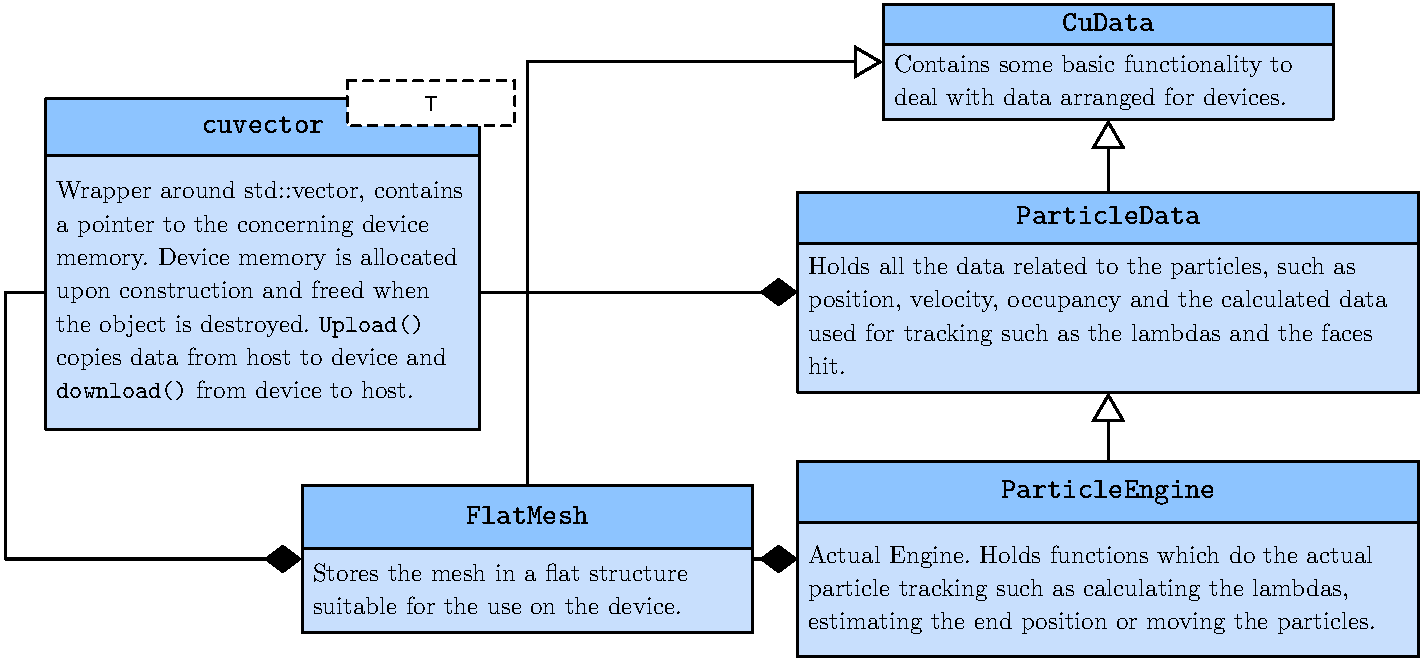
\includegraphics[scale=0.6]{content/gfx/ParticleEngineOverview.pdf}
  \caption{Simplified class diagram of the GPU tracking library.}
  \label{gfx:engineOverview}
\end{figure}

\subsection{Complete Particle Engine}

Tracking a set of particles given a start position and an (estimated) end position involves several steps. First one needs to calculate $\lambda_c$ for all particles. Recalling the equation (\ref{eq:4}) for $\lambda_c$

\begin{eqnarray}
    \lambda_{c} = \frac{(\vec{C_f} - \vec{C_c}) \bullet \vec{S_f}}{(\vec{b} - \vec{C_c}) \bullet \vec{S_f}} \nonumber
\end{eqnarray}

The only data depending on the particle to track is the end position $\vec{b}$. Therefore we can calculate the numerator of (\ref{eq:4}) in advance for every face and cell. This is done right after the mesh data is uploaded. Once $\lambda_c$ is calculated, we have a set of faces for every particle, the faces for which $\lambda_c$ is in the interval $[0,1]$. This set usually consists of zero, one or two faces.\footnote{More faces per particle can be found, but this happens not very often.} Particles for which no face was found have their end position inside the same cell in which they were at the beginning. All we need to do is move them to the end position. Therefore we need to resort the particle data and create a second set consisting of particles which still need tracking, we call this the set of remaining particles. For those, $\lambda_a$ must be calculated to figure out which face they hit. With this information all the particles can be moved: Particles not in the set of remaining particles can be moved to the end. For particles in the set of remaining particles it must be checked whether the face hit is a boundary face, and if so, the particle must be reflected at the boundary. Otherwise the particle is moved onto the face hit and the occupancy information is updated to the adjacent cell. In the next step only particles in the remaining set of this step need to be considered. Before starting with the next iteration, the velocity must be updated using the velocity vector of the new occupancy cell. This process is illustrated in figure \ref{gfx:SequenceTracking}.

\begin{figure}[H]
  \centering
  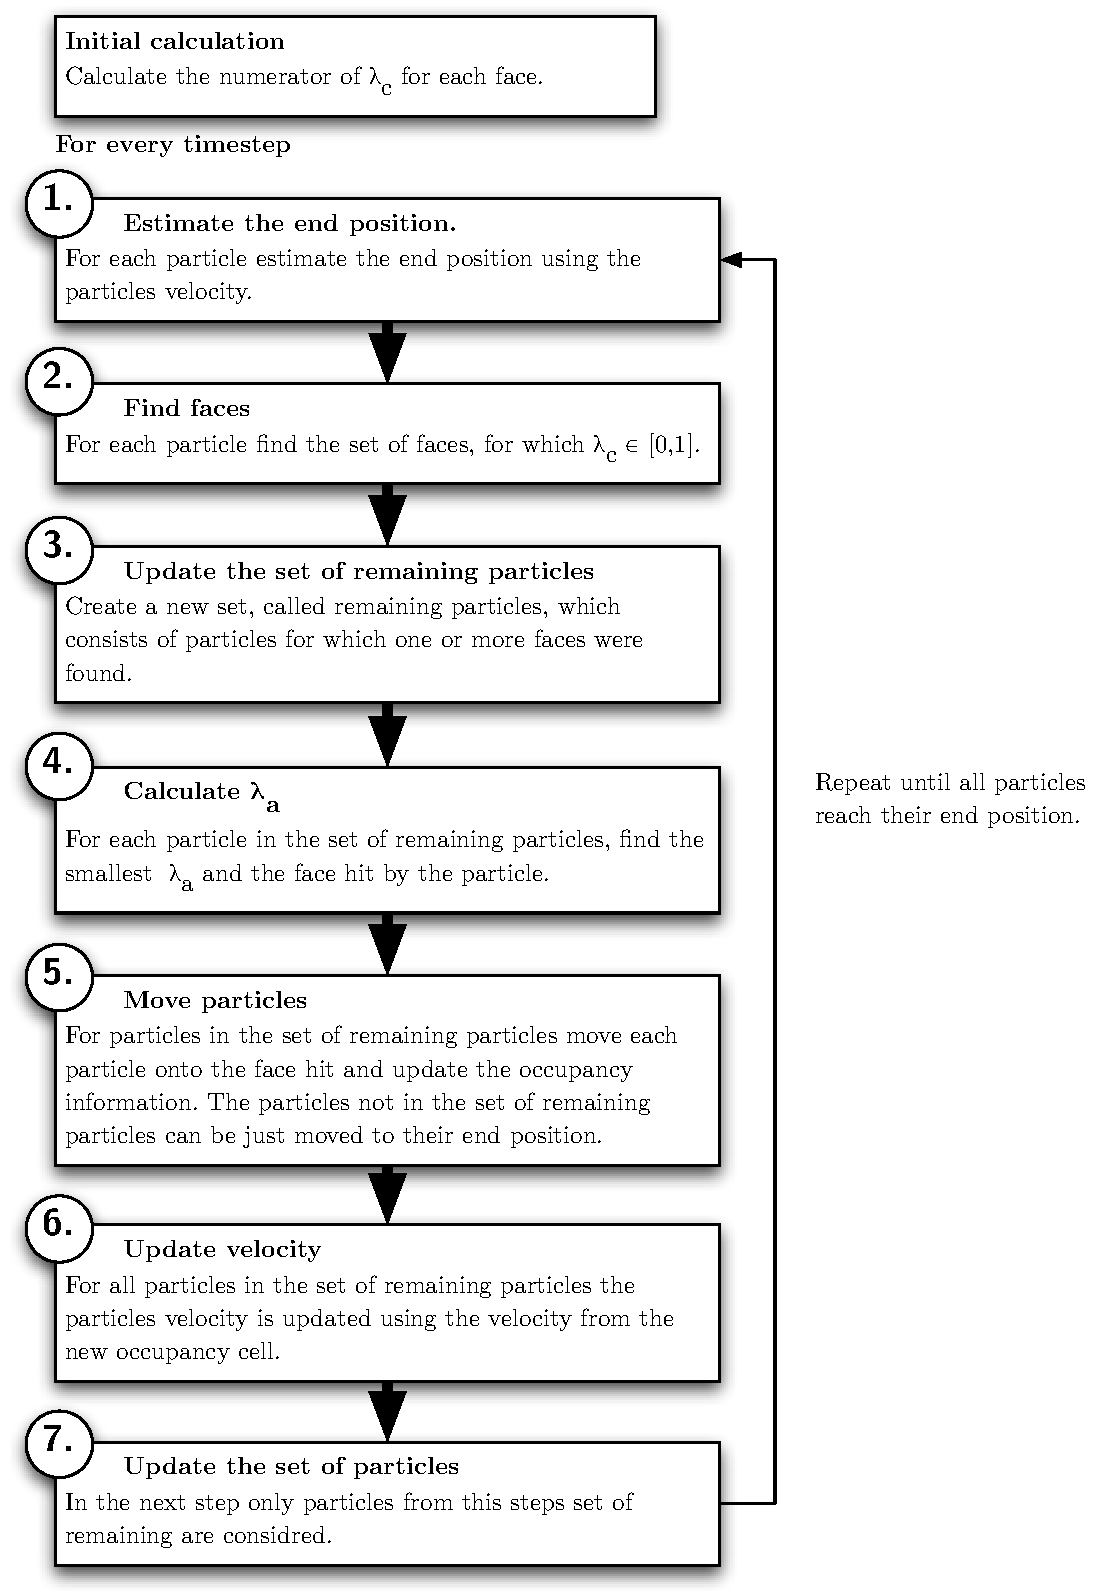
\includegraphics[scale=0.8]{content/gfx/SequenceTracking.pdf}
  \caption{Complete particle tracking sequence.}
  \label{gfx:SequenceTracking}
\end{figure}

\subsection{Data Reduction}

After calculating $\lambda_c$ it is known which particles stay in their cell. The set of particles is then reduced to the set of remaining cells using the array which holds the number of faces found as illustrated in figure \ref{gfx:reduce}.

\begin{figure}[H]
  \centering
  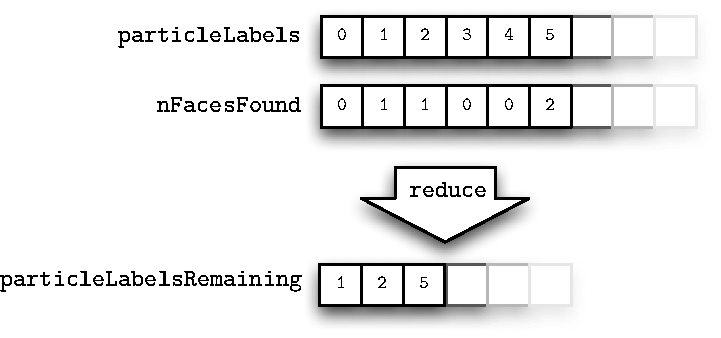
\includegraphics[scale=0.8]{content/gfx/reduce.pdf}
  \caption{Reducing the particle labels array to those which sill need tracking.}
  \label{gfx:reduce}
\end{figure}

When programming sequentially, this can be done with one simple loop. Copying the data back from the device to the host, then sort it in just one thread and upload it again takes far too much time. This is illustrated in figure \ref{gfx:widthPlotGapSort}, where the runtime of all kernel functions and memory coping is plotted. In this test, the total computing time spent on the GPU is just around 15\%. A huge part is used to copy the memory between the host and the device. The white gap shows that the GPU is idle during the time spent on the host to reduce data. The test was done on the torus (see section \ref{sec:torus}) case, where the lambdas for 100'000 particles were calculated .

\begin{figure}[H]
  \centering
  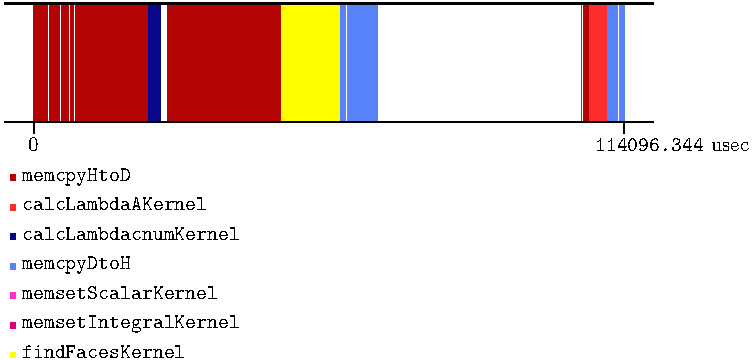
\includegraphics[scale=0.8]{content/gfx/widthPlotGapSort.pdf}
  \caption{Width plot of the GPU time spent for calculating lambdas. The CPU is used for data reduction.}
  \label{gfx:widthPlotGapSort}
\end{figure}

Doing such a reduction efficiently on massively parallel hardware is far less trivial. Fortunately sorting on the GPU is already implemented \cite{thrustRadixSort}. Thrust \cite{thrust} is a library of basic algorithms for the GPU with an interface similar to the standard template library. It includes algorithms for counting, sorting and searching. The particle labels array is reduced by the following steps on the GPU.

\begin{enumerate}
    
    \item Count the number of zeros in \verb+nFacesFound+. Use this to calculate how many particles still remain.
    
    \item Sort the \verb+particleLabels+ array using the \verb+nFacesFound+ array as key in descending order. All the labels with no faces hit will be at an index greater or equal to the number of particles remaining.
    
\end{enumerate}

\subsection{Tools and Validation}

In order to validate the results \verb+solidParticleFoam+ has been modified so that all the data going through the \verb+trackToFace(..)+ is written to the disc in binary\footnote{In a first attempt the data was just written out in text format. Because of the loss of precision it was difficult to compare the results again.} format. This includes the beginning and the end position of each particle, the cell it occupies at the beginning, the face it hits (if any) and the lambdas calculated. This data is then read by a test program, which calculates the lambdas and the faces hit again on the GPU using the start and end position stored before. The results are then compared and any differences between them is reported. This utility is called \verb+calcLambdas+ and requires the \verb+-data <dataDir>+ argument.

Doing so validates the results of the kernels which are responsible to calculate the lambdas, step 2, 3 and 4 in figure \ref{gfx:SequenceTracking}, but whether the particles are moved correctly or not is not verified. The \verb+gpuLagrangianFoam+ utility therefore comes with a switch called \verb+-validate+. If it is turned on the mesh is searched after moving the particles at the end of the time step in order to verify that the particles are in the correct cell. To generate a number of particles as test data a utility called \verb+genRandCloud+ was developed. It takes the desired number of particles as input argument and randomly positions particles in the simulation domain.

Searching the mesh is done using the octree library \cite{octree} OpenFOAM provides: The problem of finding the correct cell, given a position is reduced to the nearest neighbour problem. The centroids of all the cells in a mesh are taken as point-set and the position of the particle as the query point. The probability that the particle is in the same cell as the closest centroid is quite high and if it is not, it will be in one of the neighbouring cells. The octree is used for spatial subdivision: The bounding box of the simulation domain is recursively subdivided into 8 smaller boxes, starting from the center of the bounding box. Recursion stops once all centroids are in a separate box. During this process a tree is built which contains the direction for each step. This can be explained easier in two dimensions: Where the bounding box would be divided into 4 rectangles one at the north west, south west, north east and south east. Using this tree the program just needs to follow the direction given a position in order to solve the nearest neighbour problem.